% !TEX program = tectonic
%
% Document class choice: `acmart` sigconf mode.
% Rationale: target venues for this short (4-6pp) paper are CS-systems
% workshops that commonly accept ACM-style submissions (HotCloud, SoCC
% short papers, SYSTOR, or poster/short tracks at EuroSys). acmart also
% renders well on arXiv, which is the intended first drop. If we retarget
% to an IEEE systems venue later, swap to `\documentclass[conference]{IEEEtran}`
% and switch `\bibliographystyle{ACM-Reference-Format}` -> `IEEEtran`.
% The prior IEEEtran draft is preserved under `_archive/`.
\documentclass[sigconf,nonacm,screen]{acmart}

% --- packages ----------------------------------------------------------------
% NB: acmart preloads amsmath/amssymb/booktabs/graphicx/xcolor/url — loading
% them again here causes `\Bbbk already defined` (amssymb vs acmart math).
\usepackage{todonotes}           % flags Phase 1.1 fill-ins
\setuptodonotes{inline,color=yellow!30}

% --- metadata ----------------------------------------------------------------
\title{From Serverless to Cluster: O(1) Cache-Coherent Scraping of a
       Closed-Source Scheduling API}
\subtitle{A SETNX single-flight pattern for horizontally-replicated
          browser-automation middleware}

\author{Jess Sullivan}
\email{jess@sulliwood.org}
\affiliation{%
  \institution{Tinyland}
  \city{Ithaca}
  \state{NY}
  \country{USA}
}

% ACM-style keywords (ignored by nonacm, but useful for arXiv/indexers).
\keywords{serverless, kubernetes, cache coherence, single-flight,
          browser automation, screen scraping, scheduling}

% --- abstract ----------------------------------------------------------------
\begin{document}
\begin{abstract}
Small multi-tenant SaaS applications that depend on a closed-source
upstream (here, the Acuity Scheduling API, gated behind a paywalled
tier) are routinely forced into brittle screen-scraping over a
headless browser. A single-replica serverless deployment on Modal
handled this cost acceptably for us at $N=1$, but lifting the service
onto a three-node on-prem Kubernetes (RKE2) cluster for high
availability introduces a well-known failure mode: $N$ replicas each
populating their own in-process cache inflate upstream load by a
factor of $N$ on every TTL expiry, and cache-stampede pathologies
appear at the cold-cache edge.
We present a Redis \texttt{SETNX} single-flight pattern layered over
the existing Effect-based adapter that restores the $\mathcal{O}(1/T)$
per-cache-TTL upstream scrape cost of the original single-replica
deployment, independently of replica count $N$. We characterize the
pattern on a three-node RKE2 cluster running $N{=}2$ shadowed against
the live Modal deployment over a four-week bake, reporting scrape
counts, p99 latency, and diff-parity rates.
\todo{Fill in headline reduction number after Phase~1.1 data
      collection: target is ``$\ge (N-1)/N \cdot 100\%$ reduction in
      upstream scrapes vs.\ naive $N$-replica'', i.e.\ $\ge 50\%$ at
      $N{=}2$.}
The result is a simple, auditable coherence primitive that lets a
headless-browser middleware scale horizontally for availability
without scaling its upstream cost.
\end{abstract}

\maketitle

% =============================================================================
\section{Introduction}
\label{sec:intro}

\todo[inline]{Motivate: closed-source SaaS upstream (Acuity), no
  public API on the plan tier, brittle Playwright scraping of a
  multi-step booking wizard, need for HA as practitioner count grows.
  Set up the cost-vs-availability tension: serverless was cheap at
  $N{=}1$, but cannot meet a multi-tenant SLO. Thesis: on-prem
  Kubernetes is viable if-and-only-if cache coherence is preserved
  across replicas. Contribution list: (i) SETNX single-flight
  primitive on top of Effect, (ii) 4-week shadow-bake
  characterization against the production serverless deployment,
  (iii) an operational playbook for bounding upstream cost at
  $\mathcal{O}(1/T)$ under arbitrary replication.}

% =============================================================================
\section{Background}
\label{sec:background}

\todo[inline]{Acuity Scheduling upstream: booking-wizard anatomy,
  service-catalog shape, categories/intake-question surface areas
  that break navigation. Modal serverless runtime: cold start,
  keep-warm, per-request concurrency, single-replica determinism.
  Playwright + browser-pool constraints. Prior art we rely on:
  Memcached lease tokens \cite{nishtala-memcache-2013}, single-flight
  as folklore in Go's \texttt{singleflight} package, Redis
  \texttt{SETNX} semantics \cite{redis-setnx-docs}.}

% =============================================================================
\section{System Design}
\label{sec:design}

\todo[inline]{Architecture: Effect service graph, browser pool,
  L1 in-process + L2 Redis single-flight layer. Show the
  \texttt{RedisL2.getCached} contract (pseudocode), TTL budget, and
  the lock-winner vs.\ lock-waiter paths. Emphasize no coordination
  beyond \texttt{SETNX}. Compare to alternatives: consistent hashing
  + sticky upstream, lease-token schemes, and why SETNX is the
  minimal sufficient primitive here.}

% =============================================================================
\section{Correctness \& Complexity Analysis}
\label{sec:analysis}

\todo[inline]{Argue the invariant: for any cache key $k$ with
  TTL $T$, the expected number of upstream scrapes per second across
  $N$ replicas is $1/T + o(1)$, and is independent of $N$ in the
  stampede-free regime. Sketch the lock-timeout argument (bounded
  retry loop, no livelock under a Poisson request arrival
  assumption). Relate to cold-start literature
  \cite{lin-pool-2019,nguyen-cold-mpc-2025}.}

% =============================================================================
\section{Evaluation}
\label{sec:eval}

\todo[inline]{Phase 1.1 measurement: 4-week shadow bake, $N{=}2$
  on RKE2 vs.\ $N{=}1$ on Modal. Metrics: upstream scrape count per
  hour (Fig.~\ref{fig:scrape}), p99 slot-read latency
  (Fig.~\ref{fig:latency}), cache hit ratio (Fig.~\ref{fig:hit}).
  Diff-parity breakdown (ok / warn / critical) over the same window.
  Compare against a baseline N-naive deployment for the first 24h.}

\begin{figure}[t]
  \centering
  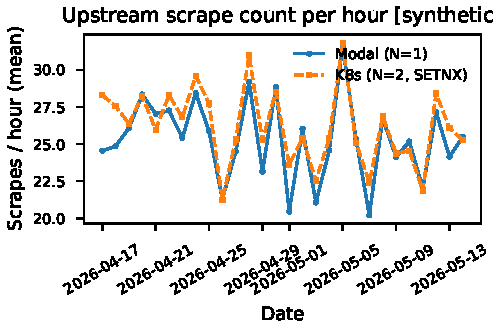
\includegraphics[width=\columnwidth]{figures/scrape_count.pdf}
  \caption{Upstream scrape count per hour during the 4-week shadow
    bake: Modal ($N{=}1$) vs.\ RKE2 ($N{=}2$) with Redis
    \texttt{SETNX} single-flight. Overlap indicates the single-flight
    preserves the $N{=}1$ cost envelope under replication.}
  \label{fig:scrape}
\end{figure}

\begin{figure}[t]
  \centering
  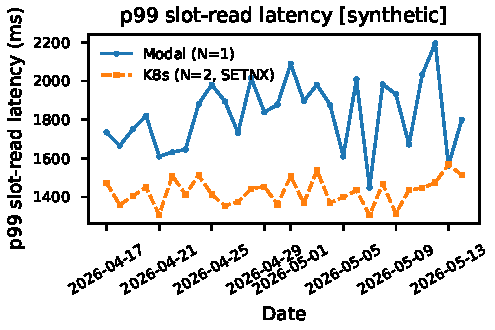
\includegraphics[width=\columnwidth]{figures/latency_p99.pdf}
  \caption{p99 end-to-end slot-read latency, Modal vs.\ RKE2.
    Lock-waiter path adds a small bounded overhead on cache-miss
    cohorts; steady-state is dominated by L1.}
  \label{fig:latency}
\end{figure}

\begin{figure}[t]
  \centering
  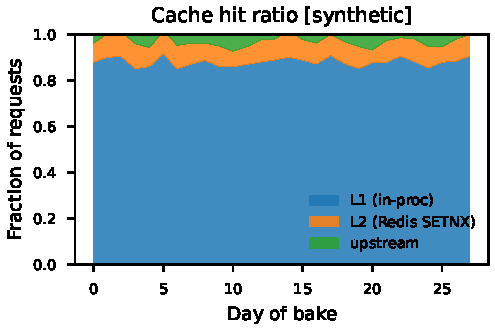
\includegraphics[width=\columnwidth]{figures/cache_hit_ratio.pdf}
  \caption{Cache hit ratio over the bake window. L1 dominates;
    L2 handles cold-replica and post-deploy windows.}
  \label{fig:hit}
\end{figure}

% =============================================================================
\section{Discussion}
\label{sec:discussion}

\todo[inline]{When does this pattern break? Upstream flakiness that
  invalidates the lock winner's result (we retry); TTL tuning
  (too-short $\Rightarrow$ stampede, too-long $\Rightarrow$ stale
  bookings); Redis partition tolerance (we tolerate brief fallback
  to L1-only). Compare to AAPA predictive autoscaling
  \cite{zhang-aapa-2025} and serverless warm-pool overhead
  \cite{kondrashov-warm-2025}.}

% =============================================================================
\section{Related Work}
\label{sec:related}

\todo[inline]{Memcache stampede control \cite{nishtala-memcache-2013};
  serverless cold-start mitigation
  \cite{lin-pool-2019,nguyen-cold-mpc-2025}; autoscaling on
  Kubernetes \cite{zhang-aapa-2025}; cost characterization of
  keep-warm policies \cite{kondrashov-warm-2025}. Contrast: our
  setting has a single closed-source upstream with no rate-limit
  API, so the cost we minimize is not dollars but risk-of-block.}

% =============================================================================
\section{Conclusion}
\label{sec:conclusion}

\todo[inline]{We restored the $\mathcal{O}(1/T)$ scrape invariant
  across $N$ replicas with $\sim 50$ LOC of Effect and a single
  Redis primitive. The pattern generalizes to any
  closed-source-upstream middleware where availability demands
  replication but cost demands coherence. Future work: multi-tenant
  generalization, predictive prewarming tied to calendar pressure.}

% --- bibliography ------------------------------------------------------------
\bibliographystyle{ACM-Reference-Format}
\bibliography{refs}

\end{document}
